\documentclass[a4paper, 11pt]{article}
\usepackage[spanish]{babel}
\selectlanguage{spanish}
\usepackage{graphicx}
\usepackage{wrapfig}
\usepackage[utf8]{inputenc}
\usepackage{amsmath}
\usepackage{dsfont}
\usepackage{multirow}
\usepackage{vmargin}
\usepackage{subfigure}
\usepackage[numbers, sort&compress]{natbib}
\usepackage{url}
\usepackage{cite}
\usepackage{wrapfig}
\usepackage{enumerate} 
\usepackage{sectsty} % centrar secciones de encabezados
\usepackage[usenames]{color}
\usepackage[dvipsnames]{xcolor}
\usepackage{fancyvrb}
\usepackage{caption}
\usepackage{amsfonts}
\usepackage{amssymb}
\usepackage{listings}
\usepackage{color}
\usepackage{algpseudocode}
\usepackage{multirow}
\usepackage[usenames]{color}
\usepackage{epstopdf}
\usepackage{float}
\usepackage{nameref}
\spanishdecimal{.}

\spanishdecimal{.}

\setmargins
{2.5cm}                        % margen izquierdo
{1cm}                         % margen superior
{16.5cm}                      % anchura del texto
{23.42cm}                    % altura del texto
{10pt}                           % altura de los encabezados
{0cm}                           % espacio entre el texto y los encabezados
{0pt}                             % altura del pie de página
{1cm}                           % espacio entre el texto y el pie de página

\definecolor{mygreen}{rgb}{0,0.6,0}
\definecolor{mygray}{rgb}{0.5,0.5,0.5}
\definecolor{mymauve}{rgb}{0.58,0,0.82}

\lstset{ 
  backgroundcolor=\color{white},   % choose the background color; you must add \usepackage{color} or \usepackage{xcolor}; should come as last argument
  basicstyle=\footnotesize,        % the size of the fonts that are used for the code
  breakatwhitespace=false,         % sets if automatic breaks should only happen at whitespace
  breaklines=true,                 % sets automatic line breaking
  captionpos=b,                    % sets the caption-position to bottom
  commentstyle=\color{mygreen},    % comment style
  deletekeywords={...},            % if you want to delete keywords from the given language
  escapeinside={\%*}{*)},          % if you want to add LaTeX within your code
  extendedchars=true,              % lets you use non-ASCII characters; for 8-bits encodings only, does not work with UTF-8
  firstnumber=1,                % start line enumeration with line 1000
  frame=single,	                   % adds a frame around the code
  keepspaces=true,                 % keeps spaces in text, useful for keeping indentation of code (possibly needs columns=flexible)
  keywordstyle=\color{blue},       % keyword style
  language=Octave,                 % the language of the code
  morekeywords={*,...},            % if you want to add more keywords to the set
  numbers=left,                    % where to put the line-numbers; possible values are (none, left, right)
  numbersep=5pt,                   % how far the line-numbers are from the code
  numberstyle=\tiny\color{mygray}, % the style that is used for the line-numbers
  rulecolor=\color{black},         % if not set, the frame-color may be changed on line-breaks within not-black text (e.g. comments (green here))
  showspaces=false,                % show spaces everywhere adding particular underscores; it overrides 'showstringspaces'
  showstringspaces=false,          % underline spaces within strings only
  showtabs=false,                  % show tabs within strings adding particular underscores
  stepnumber=1,                    % the step between two line-numbers. If it's 1, each line will be numbered
  stringstyle=\color{mymauve},     % string literal style
  tabsize=2,	                   % sets default tabsize to 2 spaces
  title=\lstname                   % show the filename of files included with \lstinputlisting; also try caption instead of title
}


\begin{document}

\title{Caracterización de la red de calidad del aire en el Área Metropolitana de Monterrey}
\author{Matr\'icula: 1985281}
\date{ }
\maketitle

\vspace{-1 cm}
\begin{center}\rule{\textwidth}{0.1mm} \end{center}
\vspace{-1.3 cm}
\begin {center}
\item \Large{\textbf{ Resumen}}
\end {center}

Recientemente, han sucedido alarmas ambientales decretadas en Monterrey sobre la mala calidad del aire, que posiciona a la ciudad como una de las más contaminadas del país, en lo que se refiere a material particulado, como el \textit{PM10} y el \textit{PM2.5}. Este trabajo esta enfocado en el problema de identificar, analizar y proponer un modelo que caracterice a la red de calidad del aire en el Área Metropolitana de Monterrey (AMM), con el fin de entender el comportamiento y evolución de esta. 

\vspace{-0.5cm}
\begin{center}\rule{\textwidth}{0.1mm} \end{center}




\section*{\centering{Introducción}}
El AMM cuenta con trece estaciones fijas de monitoreo bajo el encargo del Sistema Integral de Monitoreo Ambiental de la Secretaría de Desarrollo Sustentable  (SIMA) del Gobierno de Nuevo León, ver figura \ref{figure1}.  Los datos registrados por las estaciones de monitoreo dan una indicación de las tendencias en la calidad del aire en el AMM. En este trabajo se utilizan los datos promedios reportados del contaminante PM10 por hora de todos los días del mes de noviembre de 2017 y se predice para el mes siguiente utilizando el método de \textit{Mínimos Cuadrados Ordinarios}. Luego se establece un sistema de ecuaciones lineales con los datos encontrados por el método y se calcula el flujo de contaminación de una estación a otra.

\begin{figure}[H]
\centering
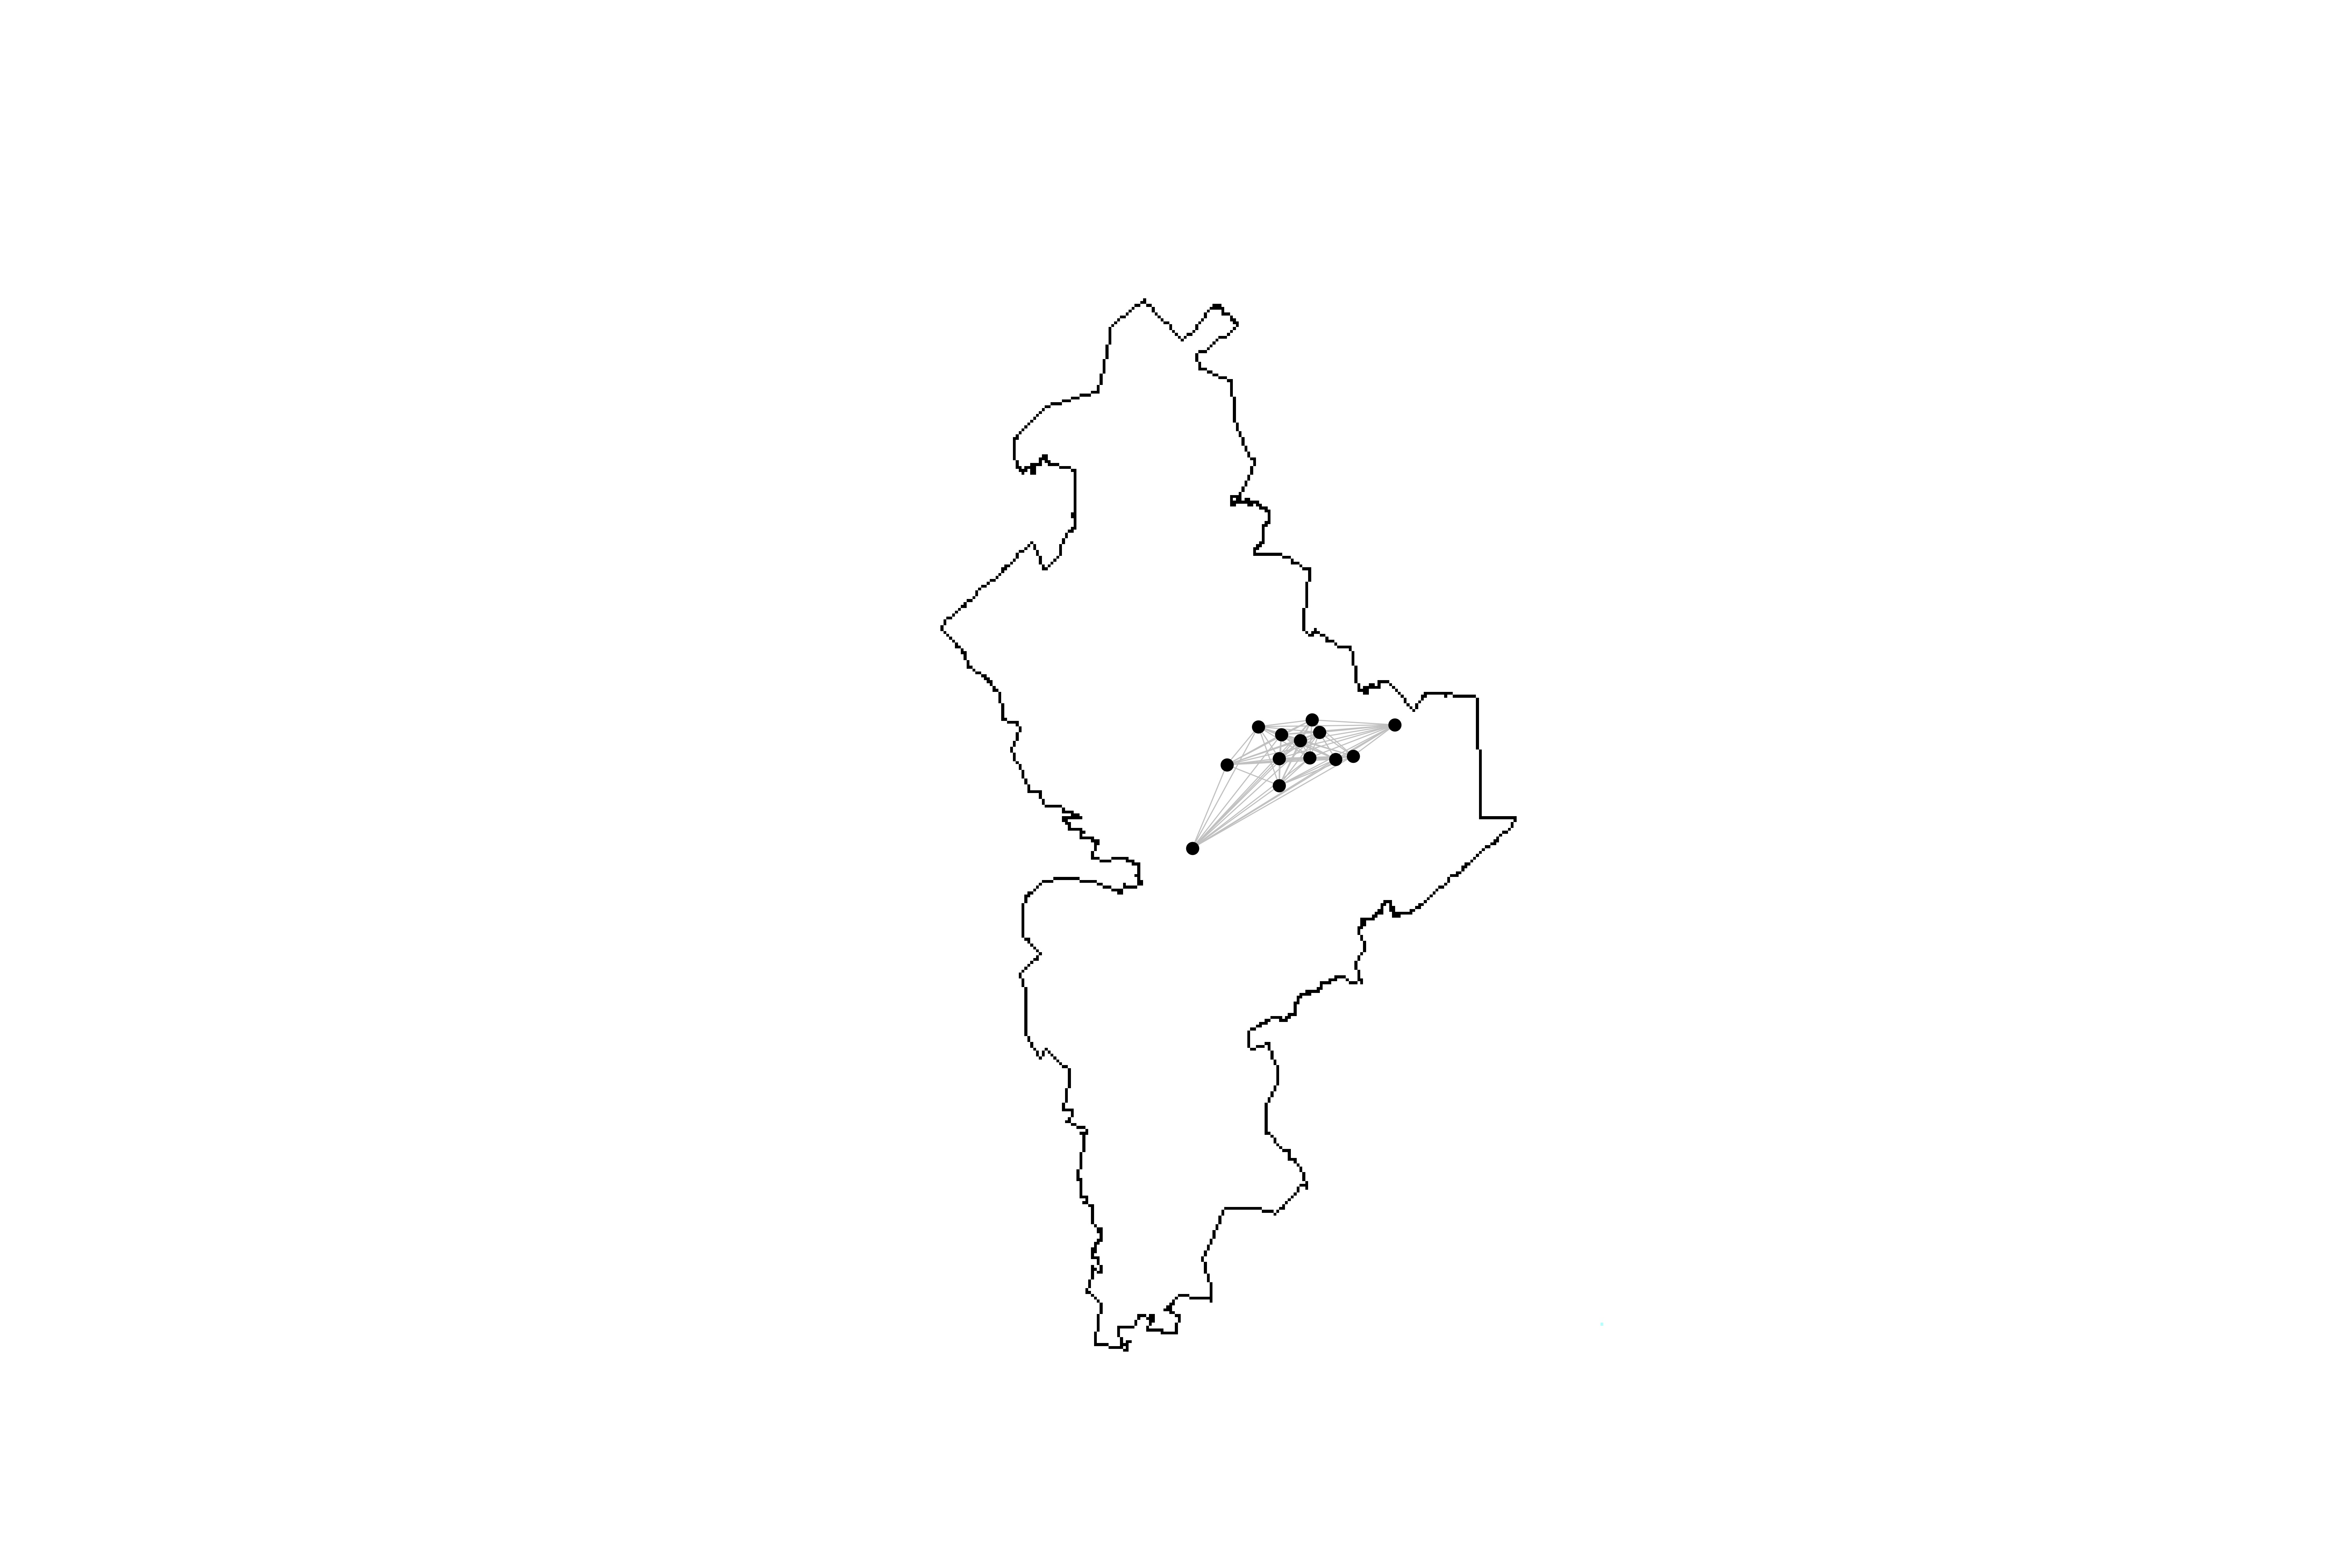
\includegraphics[width=130mm]{red_mon}
\caption{Representación de las trece estaciones de monitoreo en el AMM}
\label{figure1}
\end{figure}

\section*{\centering{Metodología y Resultados}}

Se obtienen los datos del contaminante PM10 por cada estación de monitoreo, la figura \ref{figure2} (a), representa los valores obtenidos por el contaminante PM10 durante todo el mes de noviembre en la estación Centro y la figura \ref{figure2} (b), representa los valores obtenidos por el contaminante PM10 durante todo el día 01 de noviembre de 2017 en la misma estación.
\begin{figure}[H]
\centering
\subfigure[Registro de PM10 en la estación \textit{Centro} durante noviembre de 2017]{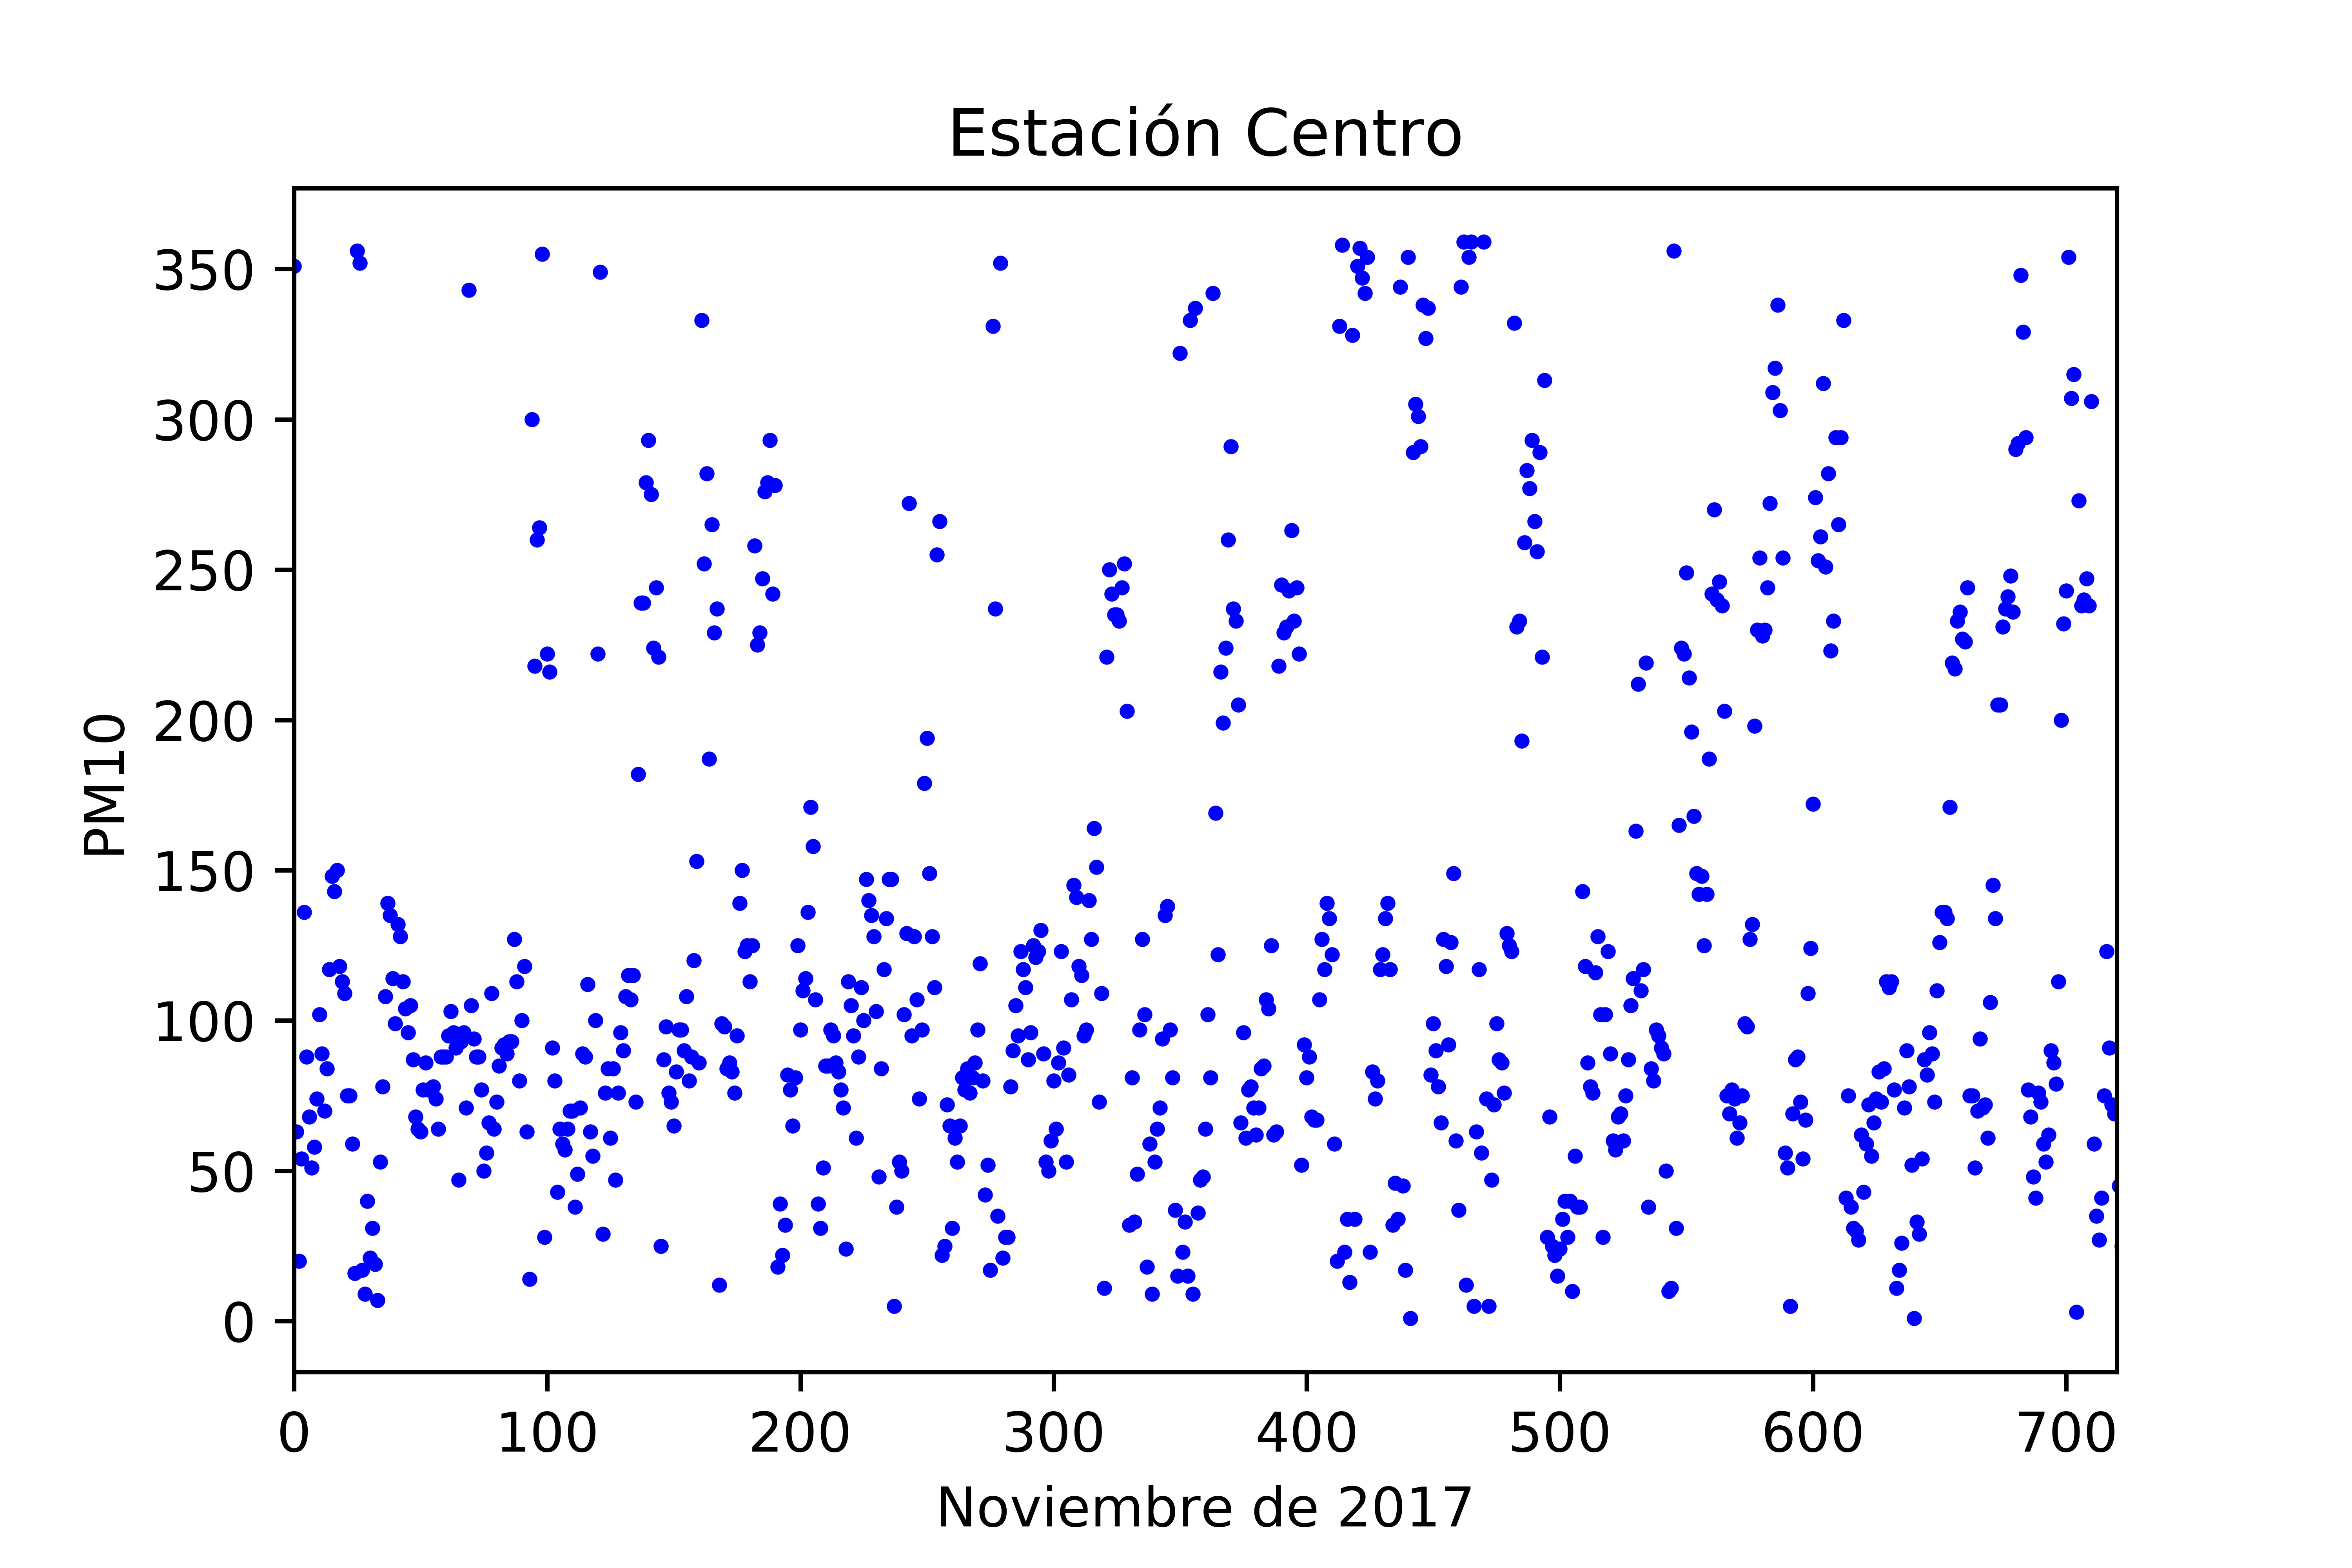
\includegraphics[width=80mm]{./11_17}}
\subfigure[Registro de PM10 en la estación \textit{Centro} durante 01 de noviembre  de 2017]{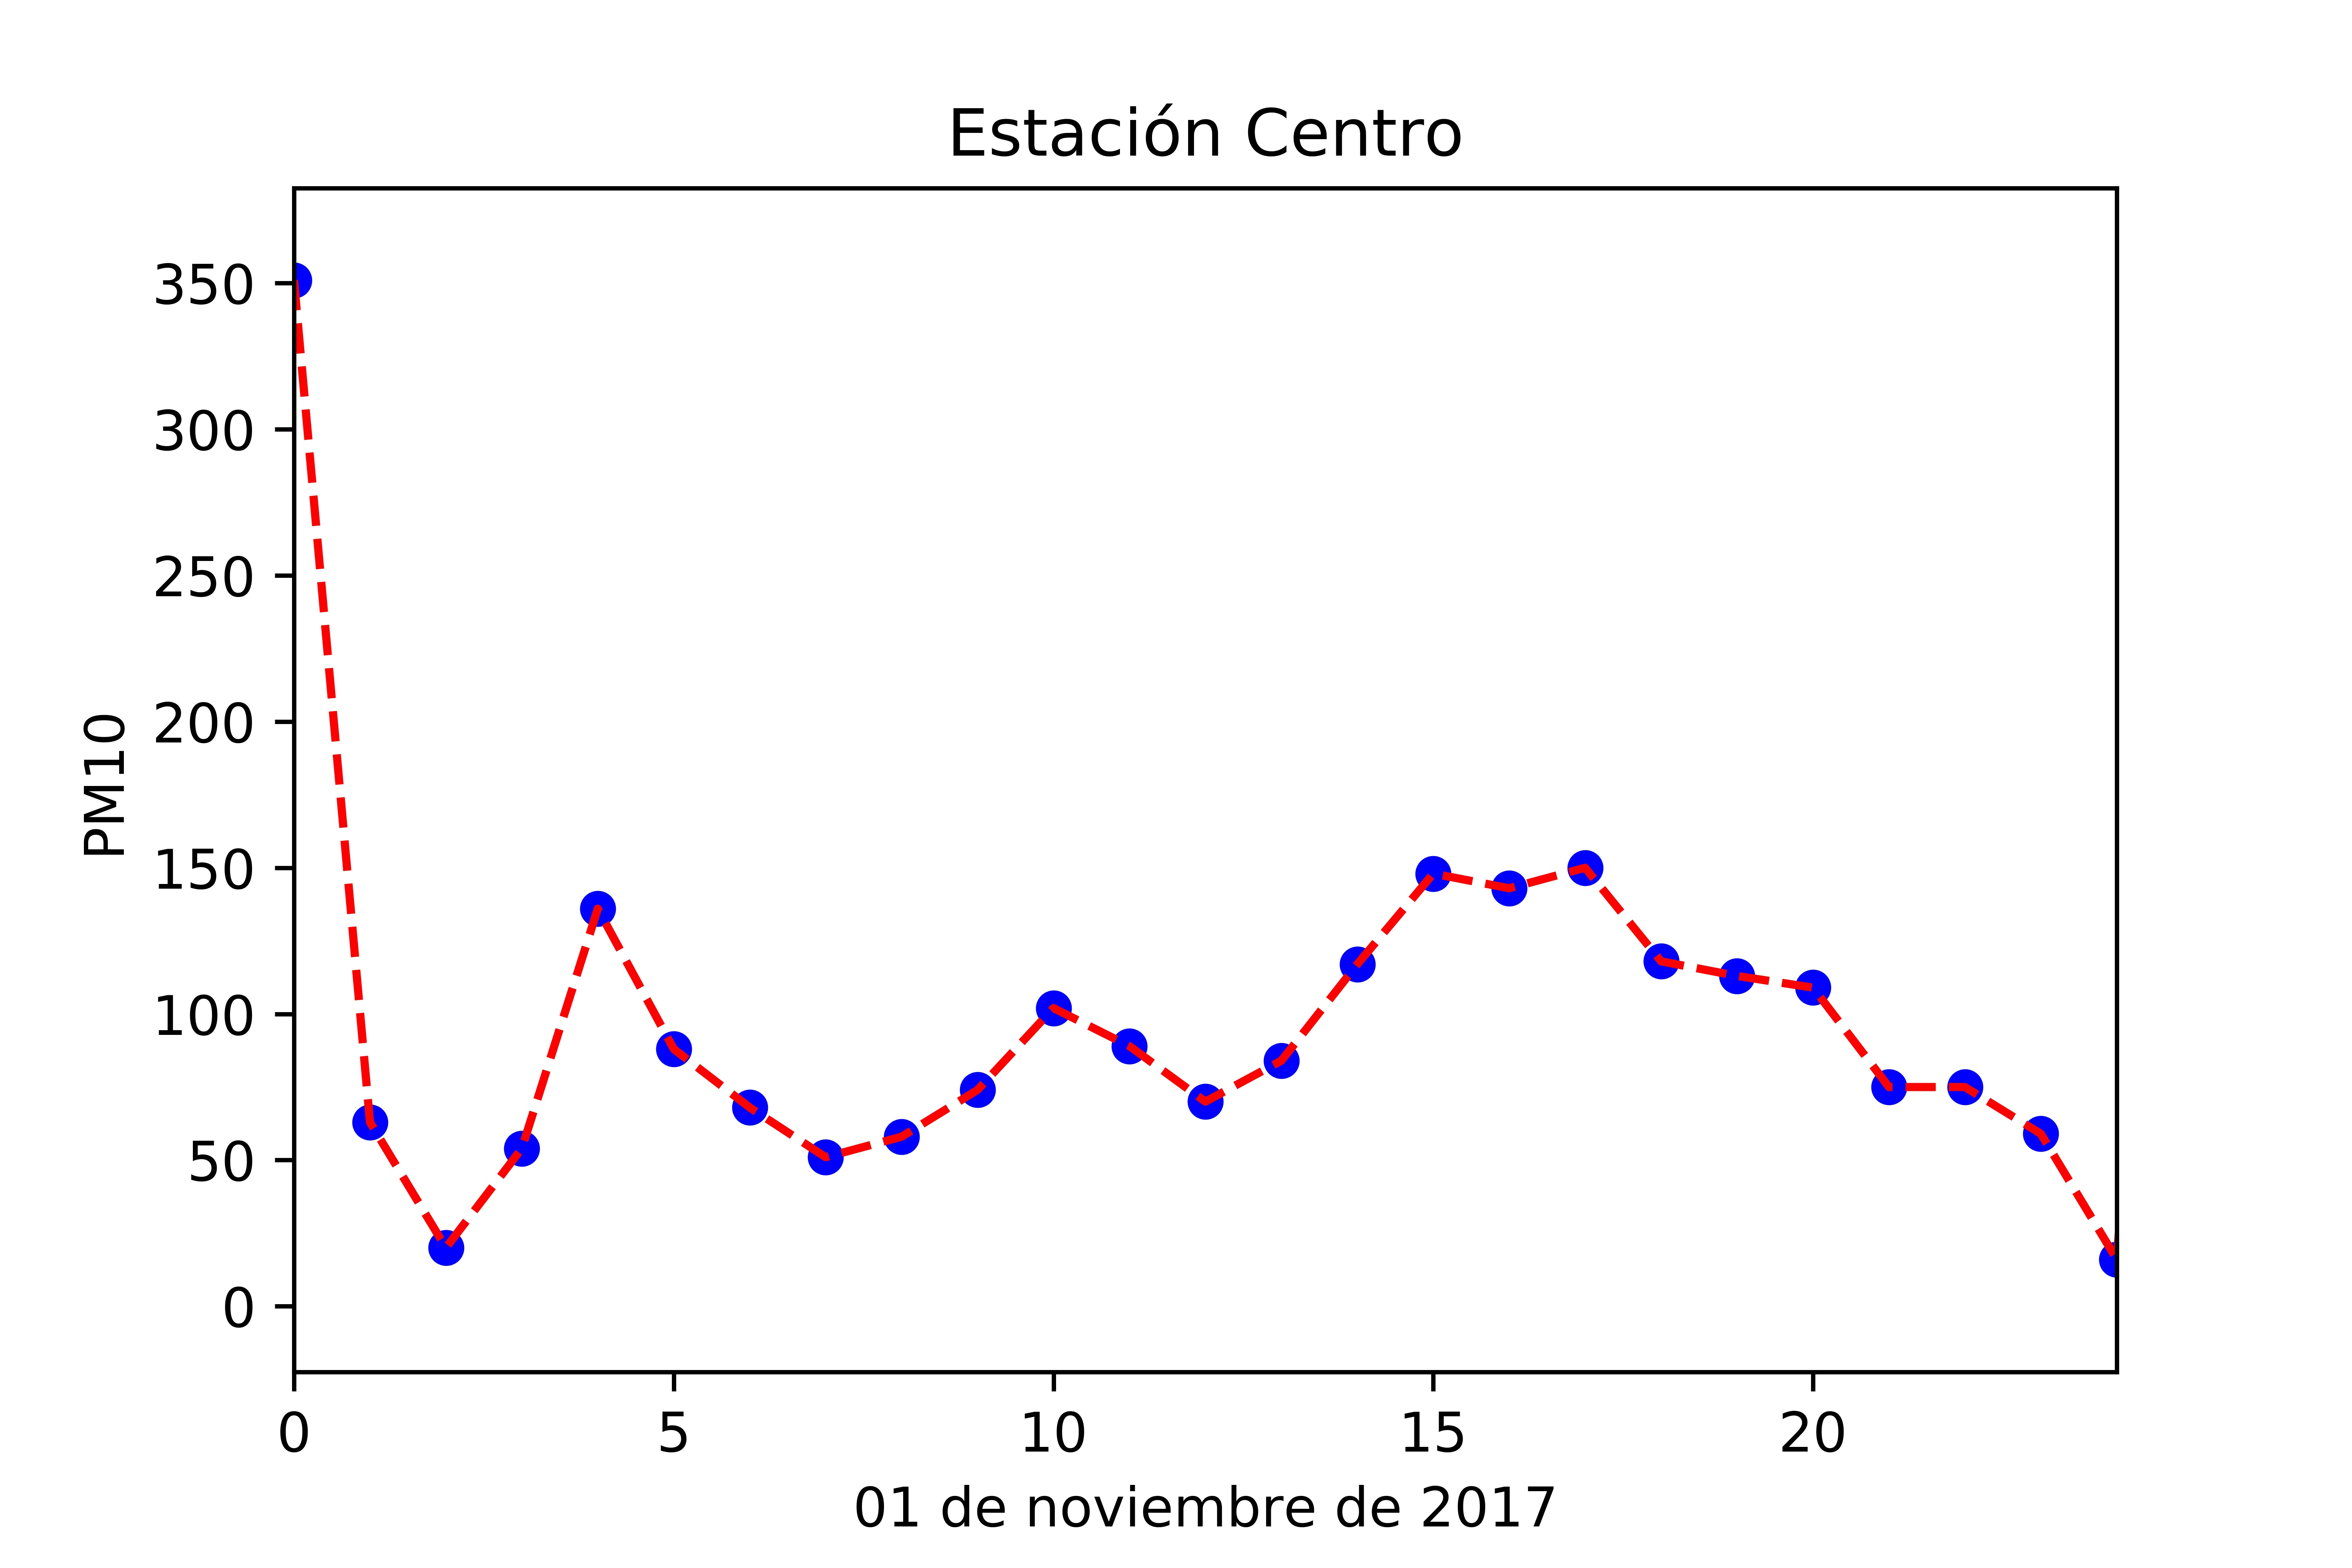
\includegraphics[width=80mm]{./01_11_17}}
\caption{Registro de PM10 en la estación \textit{Centro}}
\label{figure2}
\end{figure}

Se construye la red completa de las trece estaciones, donde los nodos representan las posiciones de las estaciones de monitoreo y las aristas representan la interación del contaminante PM10 entre éstos. A los nodos se les identifíca con un color dependiendo del nivel de contaminación que este reportando actualmente la estación de monitoreo.
\begin{figure}[H]
\centering
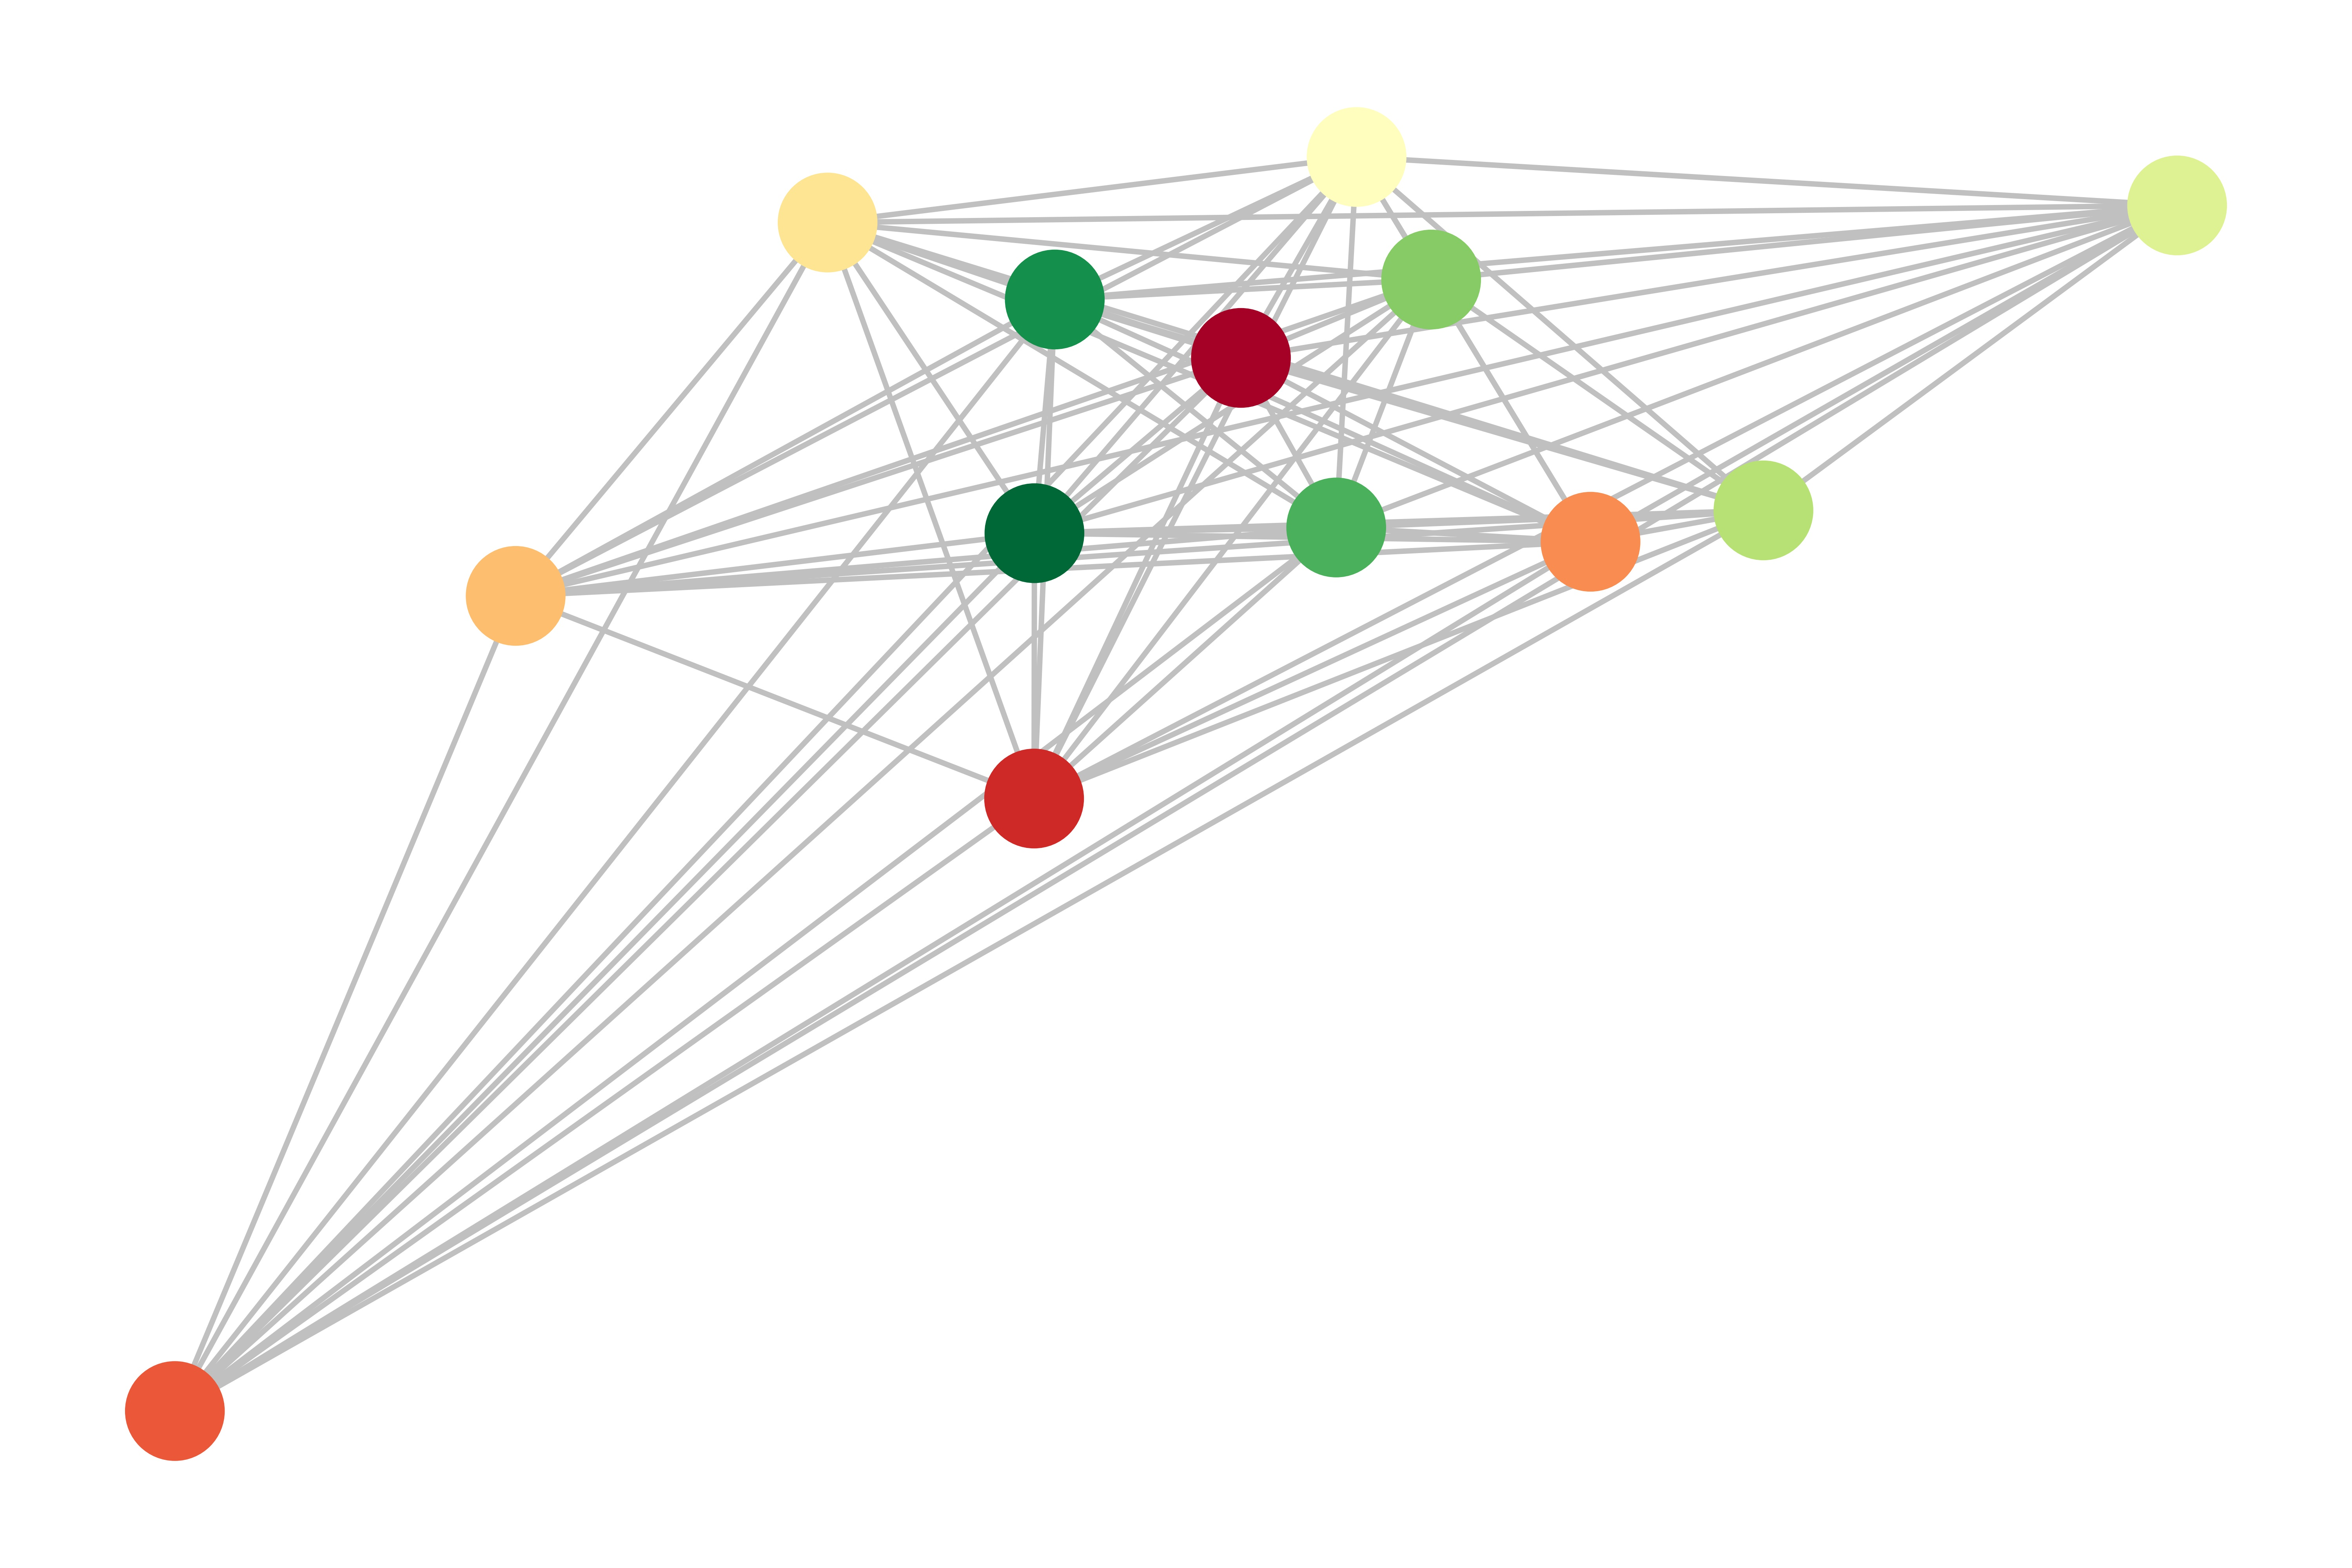
\includegraphics[width=130mm]{grafon}
\caption{Representación de las trece estaciones de monitoreo en el AMM al 01 de noviembre de 2017 a las 00:00:00 hrs. }
\label{figure3}
\end{figure}

En la figura \ref{figure3} se puede apreciar que al 01 de noviembre del 2017 la estación que reporta mayor contaminación en lo que respecta a PM10 es la estación centro, mientras que las estaciones alrededor de ella presentan registros menores de contaminante PM10 a las 00:00:00 hrs.
\\ \\
Con el método de mínimos cuadrados ordinarios se calculan los estimadores de la siguiente hora del día 01 de diciembre de 2017 (00:00:00 hrs)  para cada estación de la red de la variable de respuesta del contaminante PM10 ($e_{i}$), considerando la velocidad y la dirección del viento como variables explicativas, ver la implementación en el código para la estación Centro. 

\begin{lstlisting}[language=Python]
centro = por_estacion[0]
result = sm.ols(formula="PM10 ~ velocity + direction", data=centro).fit()
respuesta_centro = result.params[0]
\end{lstlisting}

Se calculan los pesos de las aristas ($x_{ij}$) considerando, los valores estimados ($e_{i}$), las distancias entre las estaciones ($d_{ij}$), la velocidad del viento ($v_{i}$) y las direcciones del viento ($\alpha_{i}$), de la siguiente manera:
$$ e_{i}(t+1) = \sum_{j \neq i,} ((\frac{1}{d_{ij}(t)} v_{i}(t)) + \alpha_{i}(t)) \ \ x_{ij}(t+1), \ \ \ \ \ \ \ i,j = 1, ..., 13. $$


\begin{figure}[H]
\centering
\subfigure[Calidad del aire por estación al 01 de diciembre de 2017 a las 00:00:00 hrs.]{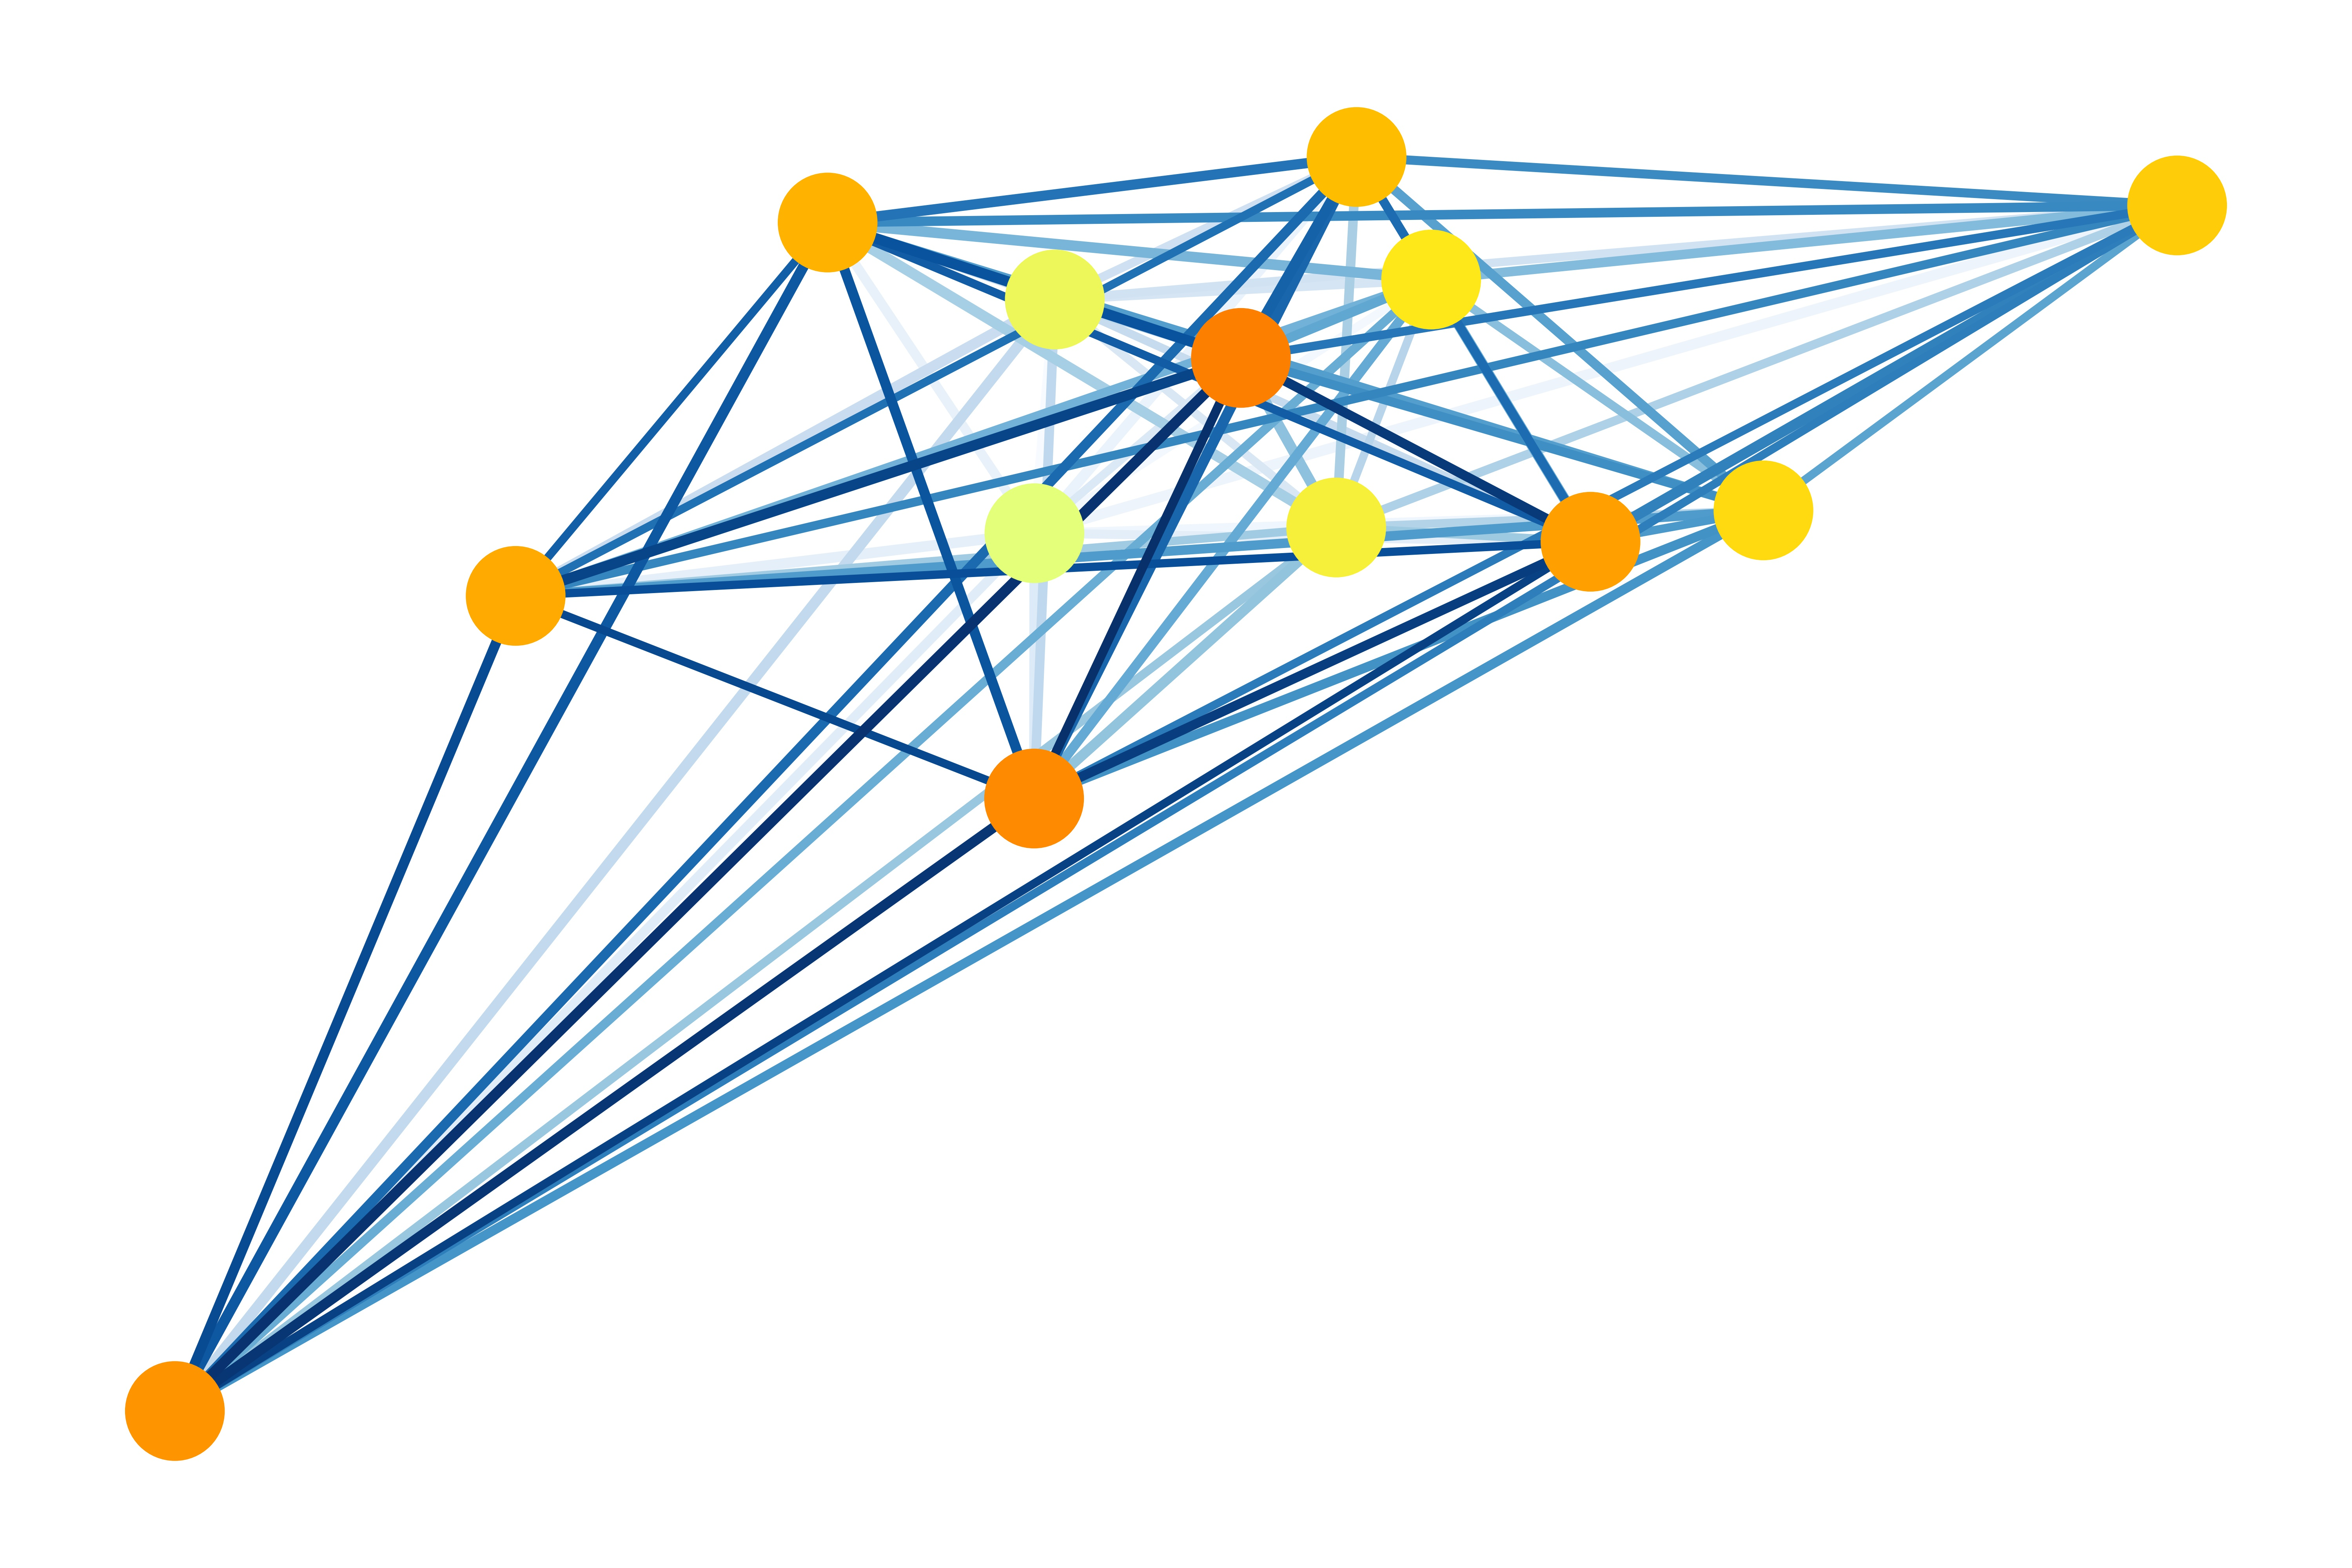
\includegraphics[width=80mm]{./grafo_cont}}
\subfigure[Rosa de viento durante noviembre de 2017 de la estación Centro]{\includegraphics[width=80mm]{./rose}}
\caption{Registro de PM10 por estación}
\label{figure4}
\end{figure}
 En la figura \ref{figure4} (a) se observa la calidad del aire en el AMM, obtenida con los valores estimados al día 01 de diciembre de 2017 a las 00:00:00 hrs. y la  \ref{figure4} (b) srepresenta la rosa de viento de la estación centro, la cual explica la dirección y velocidad del aire en esa estación.

\subsection*{Conclusiones}

Se puede concluir que la medición del contaminante PM10, esta relacionado con la velocidad y la dirección del viento, por ejemplo, en la figura \ref{figure4} (b) se observa que la dirreción del viento corre de este a oeste, sin embargo la velocidad con la que llega a ese punto es menor que con la que sale, esto indica que hay propiedades topológicas que modifican la valocidad del viento haciendo que sea más lento y que haya una mayor concentración de particulas PM10 en la estación Centro. Al comparar con lo obtenido por los estimadores podemos ver en la figura  \ref{figure4} (a) que las estaciones al este de la estación centro reportan una menor contaminación de PM10, lo que quiere decir que el viento es causante de la interacción entre contaminantes de la red, mientras que la estación Centro reporta un alto registro de particulas PM10. Támbien se puede observar que las estaciones al oeste de la estación Centro reportan aún menores índices de contaminante que  la estación Centro lo que indica que el principal factor es la velocidad del aire.


\bibliographystyle{unsrt}
\bibliography{biblio}
\nocite{*}

\end{document}